\documentclass[11pt,a4paper]{report}
\usepackage[textwidth=37em,vmargin=30mm]{geometry}
\usepackage{calc,xunicode,amsmath,amssymb,paralist,enumitem,tabu,booktabs,datetime2,xeCJK,xeCJKfntef,listings}
\usepackage{tocloft,fancyhdr,tcolorbox,xcolor,graphicx,eso-pic,xltxtra,xelatexemoji}

\newcommand{\envyear}[0]{2025}
\newcommand{\envdatestr}[0]{2025-05-21}
\newcommand{\envfinaldir}[0]{webdb/2025/20250521/final}

\usepackage[hidelinks]{hyperref}
\hypersetup{
    colorlinks=false,
    pdfpagemode=FullScreen,
    pdftitle={Web Digest - \envdatestr}
}

\setlength{\cftbeforechapskip}{10pt}
\renewcommand{\cftchapfont}{\rmfamily\bfseries\large\raggedright}
\setlength{\cftbeforesecskip}{2pt}
\renewcommand{\cftsecfont}{\sffamily\small\raggedright}

\setdefaultleftmargin{2em}{2em}{1em}{1em}{1em}{1em}

\usepackage{xeCJK,xeCJKfntef}
\xeCJKsetup{PunctStyle=plain,RubberPunctSkip=false,CJKglue=\strut\hskip 0pt plus 0.1em minus 0.05em,CJKecglue=\strut\hskip 0.22em plus 0.2em}
\XeTeXlinebreaklocale "zh"
\XeTeXlinebreakskip = 0pt


\setmainfont{Brygada 1918}
\setromanfont{Brygada 1918}
\setsansfont{IBM Plex Sans}
\setmonofont{JetBrains Mono NL}
\setCJKmainfont{Noto Serif CJK SC}
\setCJKromanfont{Noto Serif CJK SC}
\setCJKsansfont{Noto Sans CJK SC}
\setCJKmonofont{Noto Sans CJK SC}

\setlength{\parindent}{0pt}
\setlength{\parskip}{8pt}
\linespread{1.15}

\lstset{
	basicstyle=\ttfamily\footnotesize,
	numbersep=5pt,
	backgroundcolor=\color{black!5},
	showspaces=false,
	showstringspaces=false,
	showtabs=false,
	tabsize=2,
	captionpos=b,
	breaklines=true,
	breakatwhitespace=true,
	breakautoindent=true,
	linewidth=\textwidth
}






\newcommand{\coverpic}[2]{
    % argv: itemurl, authorname
    Cover photo by #2~~(\href{#1}{#1})
}
\newcommand{\makeheader}[0]{
    \begin{titlepage}
        % \newgeometry{hmargin=15mm,tmargin=21mm,bmargin=12mm}
        \begin{center}
            
            \rmfamily\scshape
            \fontspec{BaskervilleF}
            \fontspec{Old Standard}
            \fontsize{59pt}{70pt}\selectfont
            WEB\hfill DIGEST
            
            \vfill
            % \vskip 30pt
            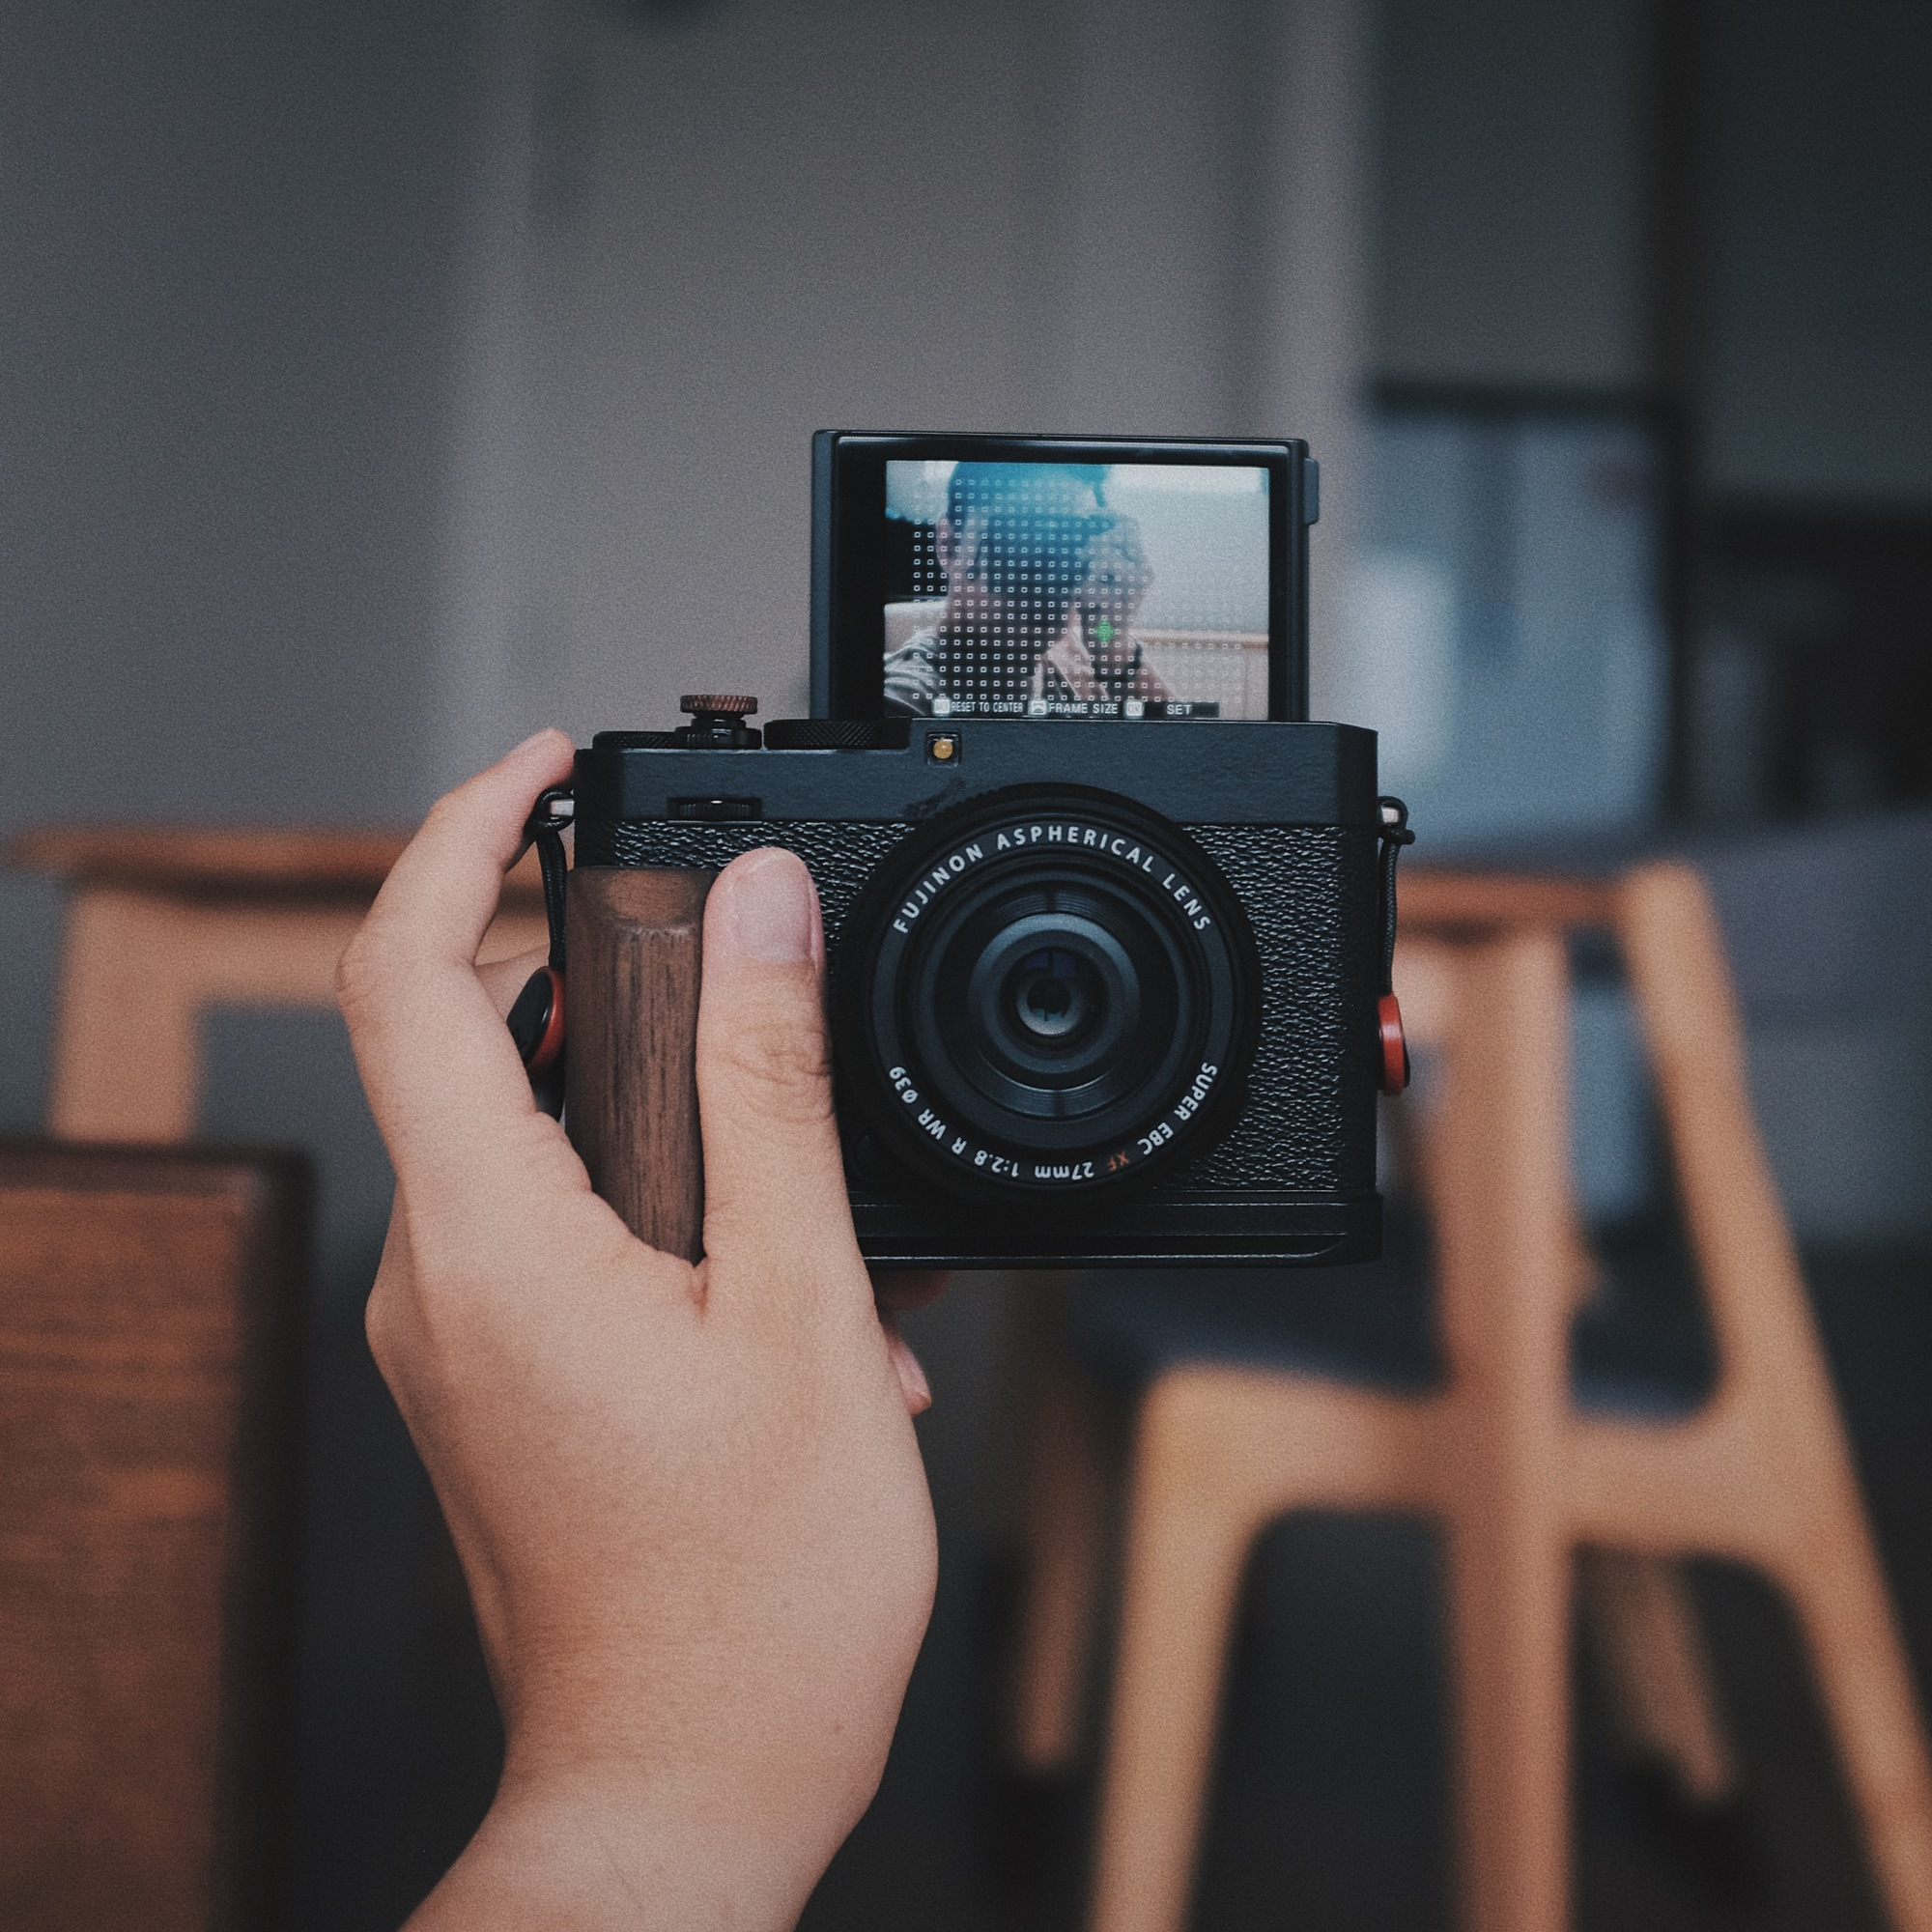
\includegraphics[width=\linewidth]{\envfinaldir/coverpic-prod.jpg}\par
            % \vskip 30pt
            \vfill

            \normalsize\rmfamily\scshape
            \copyright{} The Web Digest Project \hfill\large \envdatestr
        \end{center}
    \end{titlepage}
    % \restoregeometry
}
\newcommand{\simplehref}[1]{%
    \textcolor{blue!80!green}{\href{#1}{#1}}%
}
\renewcommand{\contentsname}{\center\Huge\sffamily\bfseries Contents\par\vskip 20pt}
\newcounter{ipartcounter}
\setcounter{ipartcounter}{0}
\newcommand{\ipart}[1]{
    % \vskip 20pt
    \clearpage
    \stepcounter{ipartcounter}
    \phantomsection
    \addcontentsline{toc}{chapter}{#1}
    % \begin{center}
    %     \Huge
    %     \sffamily\bfseries
    %     #1
    % \end{center}
    % \vskip 20pt plus 7pt
}
\newcounter{ichaptercounter}
\setcounter{ichaptercounter}{0}
\newcommand{\ichapter}[1]{
    % \vskip 20pt
    \clearpage
    \stepcounter{ichaptercounter}
    \phantomsection
    \addcontentsline{toc}{section}{\numberline{\arabic{ichaptercounter}}#1}
    \begin{center}
        \Huge
        \sffamily\bfseries
        #1
    \end{center}
    \vskip 20pt plus 7pt
}
\newcommand{\entrytitlefont}[1]{\subsection*{\raggedright\Large\sffamily\bfseries#1}}
\newcommand{\entryitemGeneric}[2]{
    % argv: title, url
    \parbox{\linewidth}{
        \entrytitlefont{#1}\par\vskip 5pt
        \footnotesize\ttfamily\mdseries
        \simplehref{#2}
    }\vskip 11pt plus 11pt minus 1pt
}
\newcommand{\entryitemGithub}[3]{
    % argv: title, url, desc
    \parbox{\linewidth}{
        \entrytitlefont{#1}\par\vskip 5pt
        \footnotesize\ttfamily\mdseries
        \simplehref{#2}\par\vskip 5pt
        \small\rmfamily\mdseries#3
    }\vskip 11pt plus 11pt minus 1pt
}
\newcommand{\entryitemAp}[3]{
    % argv: title, url, desc
    \parbox{\linewidth}{
        \entrytitlefont{#1}\par\vskip 5pt
        \footnotesize\ttfamily\mdseries
        \simplehref{#2}\par\vskip 5pt
        \small\rmfamily\mdseries#3
    }\vskip 11pt plus 11pt minus 1pt
}
\newcommand{\entryitemHackernews}[3]{
    % argv: title, hnurl, rawurl
    % \parbox{\linewidth}{
    %     \entrytitlefont{#1}\par\vskip 5pt
    %     \footnotesize\ttfamily\mdseries
    %     \simplehref{#3}\par
    %     \textcolor{black!50}{\href{#2}{#2}}
    % }\vskip 11pt plus 11pt minus 1pt
    \begin{minipage}{\linewidth}
            \entrytitlefont{#1}\par\vskip 5pt
            \footnotesize\ttfamily\mdseries
            \simplehref{#3}\par
            \textcolor{black!50}{\href{#2}{#2}}
    \end{minipage}\par\vskip 11pt plus 11pt minus 1pt
}







\begin{document}

\makeheader

\tableofcontents\clearpage




\ipart{Developers}
\ichapter{Hacker News}
\entryitemTwoLinks{Litestream: Revamped}{https://news.ycombinator.com/item?id=44045292}{https://fly.io/blog/litestream-revamped/}

\entryitemTwoLinks{The NSA Selector}{https://news.ycombinator.com/item?id=44044459}{https://github.com/wenzellabs/the\_NSA\_selector}

\entryitemTwoLinks{Gemma 3n preview: Mobile-first AI}{https://news.ycombinator.com/item?id=44044451}{https://developers.googleblog.com/en/introducing-gemma-3n/}

\entryitemTwoLinks{Google AI Ultra}{https://news.ycombinator.com/item?id=44044367}{https://blog.google/products/google-one/google-ai-ultra/}

\entryitemTwoLinks{Gemma 3n preview: Mobile-first AI}{https://news.ycombinator.com/item?id=44044199}{https://developers.googleblog.com/en/introducing-gemma-3n/}

\entryitemTwoLinks{Veo 3 and Imagen 4, and a new tool for filmmaking called Flow}{https://news.ycombinator.com/item?id=44044043}{https://blog.google/technology/ai/generative-media-models-io-2025/}

\entryitemTwoLinks{The Dawn of Nvidia's Technology}{https://news.ycombinator.com/item?id=44043687}{https://blog.dshr.org/2025/05/the-dawn-of-nvidias-technology.html}

\entryitemTwoLinks{Robin: A multi-agent system for automating scientific discovery}{https://news.ycombinator.com/item?id=44043323}{https://arxiv.org/abs/2505.13400}

\entryitemTwoLinks{Show HN: A Tiling Window Manager for Windows, Written in Janet}{https://news.ycombinator.com/item?id=44042490}{https://agent-kilo.github.io/jwno/}

\entryitemTwoLinks{Show HN: 90s.dev – Game maker that runs on the web}{https://news.ycombinator.com/item?id=44042371}{https://90s.dev/blog/finally-releasing-90s-dev.html}

\entryitemTwoLinks{OpenAI Codex hands-on review}{https://news.ycombinator.com/item?id=44042070}{https://zackproser.com/blog/openai-codex-review}

\entryitemTwoLinks{Deep Learning Is Applied Topology}{https://news.ycombinator.com/item?id=44041738}{https://theahura.substack.com/p/deep-learning-is-applied-topology}

\entryitemTwoLinks{Why Does the U.S. Always Run a Trade Deficit?}{https://news.ycombinator.com/item?id=44040407}{https://libertystreeteconomics.newyorkfed.org/2025/05/why-does-the-u-s-always-run-a-trade-deficit/}

\entryitemTwoLinks{Reports of Deno's Demise Have Been Greatly Exaggerated}{https://news.ycombinator.com/item?id=44040332}{https://deno.com/blog/greatly-exaggerated}

\entryitemTwoLinks{The emoji problem (2022)}{https://news.ycombinator.com/item?id=44039864}{https://artofproblemsolving.com/community/c2532359h2760821\_the\_emoji\_problem\_\_part\_i?srsltid=AfmBOor9TbMq\_A7hGHSJGfoWaa2HNzducSYZu35d\_LFlCSNLXpvt-pdS}

\entryitemTwoLinks{A simple search engine from scratch}{https://news.ycombinator.com/item?id=44039744}{https://bernsteinbear.com/blog/simple-search/}

\entryitemTwoLinks{The behavior of LLMs in hiring decisions: Systemic biases in candidate selection}{https://news.ycombinator.com/item?id=44039563}{https://davidrozado.substack.com/p/the-strange-behavior-of-llms-in-hiring}

\entryitemTwoLinks{Finland announces migration of its rail network to international gauge}{https://news.ycombinator.com/item?id=44038835}{https://yle.fi/a/74-20161606}

\entryitemTwoLinks{Making video games (without an engine) in 2025}{https://news.ycombinator.com/item?id=44038209}{https://noelberry.ca/posts/making\_games\_in\_2025/}

\entryitemTwoLinks{AI in my plasma physics research didn't go the way I expected}{https://news.ycombinator.com/item?id=44037941}{https://www.understandingai.org/p/i-got-fooled-by-ai-for-science-hypeheres}\ichapter{Phoronix}
\entryitemGeneric{\hskip 0pt{}Linux Scheduler Patches Aim To Address Performance Regression Since Last Year}{https://www.phoronix.com/news/Linux-Sched-Fixing-Post-611-RFC}

\entryitemGeneric{\hskip 0pt{}Fedora 43 Cleared To Ship With Wayland-Only GNOME}{https://www.phoronix.com/news/Fedora-43-Wayland-Only-GNOME}

\entryitemGeneric{\hskip 0pt{}Red Hat \& AMD Collaborating To Further Enhance Open-Source GPU Stack For AI}{https://www.phoronix.com/news/Red-Hat-AMD-Collaborating-2025}

\entryitemGeneric{\hskip 0pt{}Red Hat Announces The llm-d Open-Source Project For Gen AI}{https://www.phoronix.com/news/Red-Hat-llm-d-AI-LLM-Project}

\entryitemGeneric{\hskip 0pt{}Some Minor Performance Hits Observed With New Intel Arrow Lake 0x118 CPU Microcode}{https://www.phoronix.com/news/Intel-Arrow-Lake-0x118}

\entryitemGeneric{\hskip 0pt{}LibreOffice 25.8 Alpha 1 Released With Performance Optimizations}{https://www.phoronix.com/news/LibreOffice-25.8-Alpha-1}

\entryitemGeneric{\hskip 0pt{}Red Hat Enterprise Linux 10.0 Formally Announced, Joined By RISC-V Developer Preview}{https://www.phoronix.com/news/Red-Hat-Enterprise-Linux-10.0}

\entryitemGeneric{\hskip 0pt{}VKD3D 1.16 Released With DXIL Shader Support}{https://www.phoronix.com/news/VKD3D-1.16-Released}

\entryitemGeneric{\hskip 0pt{}Adaptive Sharpness Property Still Being Worked On For Intel Lunar Lake \& Newer On Linux}{https://www.phoronix.com/news/DRM-Sharpness-Prop-May-2025}\ichapter{Dribbble}
\entryitemGeneric{\hskip 0pt{}DICH™ Fashion Vol.2}{https://dribbble.com/shots/26046875-DICH-Fashion-Vol-2}

\entryitemGeneric{\hskip 0pt{}Mackerel}{https://dribbble.com/shots/26043994-Mackerel}

\entryitemGeneric{\hskip 0pt{}Evergreen}{https://dribbble.com/shots/26042187-Evergreen}

\entryitemGeneric{\hskip 0pt{}Howdy from a happy hermit!}{https://dribbble.com/shots/26043217-Howdy-from-a-happy-hermit}

\entryitemGeneric{\hskip 0pt{}F}{https://dribbble.com/shots/26041370-F}

\entryitemGeneric{\hskip 0pt{}Dark or Light?}{https://dribbble.com/shots/26042325-Dark-or-Light}

\entryitemGeneric{\hskip 0pt{}QueenClub Logo Design}{https://dribbble.com/shots/26042947-QueenClub-Logo-Design}

\entryitemGeneric{\hskip 0pt{}Ebay Rebranding Concept}{https://dribbble.com/shots/26039712-Ebay-Rebranding-Concept}

\entryitemGeneric{\hskip 0pt{}Profile Card 👧}{https://dribbble.com/shots/26033069-Profile-Card}

\entryitemGeneric{\hskip 0pt{}DICH™ Fashion}{https://dribbble.com/shots/26032014-DICH-Fashion}

\entryitemGeneric{\hskip 0pt{}Techtots on UI8 illustration set}{https://dribbble.com/shots/25995896-Techtots-on-UI8-illustration-set}

\entryitemGeneric{\hskip 0pt{}Letter E + Link Logo Concept}{https://dribbble.com/shots/26032100-Letter-E-Link-Logo-Concept}

\entryitemGeneric{\hskip 0pt{}East Meats West}{https://dribbble.com/shots/26027917-East-Meats-West}

\entryitemGeneric{\hskip 0pt{}Assist Logo Design (Unused for Sale)}{https://dribbble.com/shots/26027053-Assist-Logo-Design-Unused-for-Sale}

\entryitemGeneric{\hskip 0pt{}Goldfish Concept}{https://dribbble.com/shots/26029115-Goldfish-Concept}

\entryitemGeneric{\hskip 0pt{}Matte Glass Logo}{https://dribbble.com/shots/26027999-Matte-Glass-Logo}

\entryitemGeneric{\hskip 0pt{}Sellin dashboard}{https://dribbble.com/shots/26027518-Sellin-dashboard}

\entryitemGeneric{\hskip 0pt{}Healthcare Dashboard UI/UX Design}{https://dribbble.com/shots/26026655-Healthcare-Dashboard-UI-UX-Design}

\entryitemGeneric{\hskip 0pt{}Type Illustration}{https://dribbble.com/shots/26023946-Type-Illustration}

\entryitemGeneric{\hskip 0pt{}B2B Dashboard \& Web App UI UX Design for Carbon Solutions}{https://dribbble.com/shots/25993068-B2B-Dashboard-Web-App-UI-UX-Design-for-Carbon-Solutions}

\entryitemGeneric{\hskip 0pt{}Web3 crypto hero section 3d motion design}{https://dribbble.com/shots/26017311-Web3-crypto-hero-section-3d-motion-design}

\entryitemGeneric{\hskip 0pt{}Recent Marks \& Lettermarks}{https://dribbble.com/shots/26023308-Recent-Marks-Lettermarks}

\entryitemGeneric{\hskip 0pt{}Cat and Dog Brand Mascots}{https://dribbble.com/shots/26023569-Cat-and-Dog-Brand-Mascots}

\entryitemGeneric{\hskip 0pt{}Apefilm logo}{https://dribbble.com/shots/26021962-Apefilm-logo}


\ipart{Developers~~~~(zh-Hans)}
\ichapter{Solidot}
\entryitemGeneric{\hskip 0pt{}人体肺活量衰减始于 20-25 岁}{https://www.solidot.org/story?sid=81339}

\entryitemGeneric{\hskip 0pt{}7-Eleven 在东京都地区测试机器人送货}{https://www.solidot.org/story?sid=81338}

\entryitemGeneric{\hskip 0pt{}分数量子反常霍尔效应}{https://www.solidot.org/story?sid=81337}

\entryitemGeneric{\hskip 0pt{}微软开源 Windows Subsystem for Linux}{https://www.solidot.org/story?sid=81336}

\entryitemGeneric{\hskip 0pt{}DDoSecrets 发布窃取自 TeleMessage 的 410 GB 数据集}{https://www.solidot.org/story?sid=81335}

\entryitemGeneric{\hskip 0pt{}Firefox 快速释出更新修复两个 Pwn2Own 上公开的漏洞利用}{https://www.solidot.org/story?sid=81334}

\entryitemGeneric{\hskip 0pt{}oniux:为 Linux 应用提供 Tor 网络隔离}{https://www.solidot.org/story?sid=81333}

\entryitemGeneric{\hskip 0pt{}民主国家更环保但将污染外包给非民主国家}{https://www.solidot.org/story?sid=81332}

\entryitemGeneric{\hskip 0pt{}早期亚洲人完成了人类最长的史前迁徙}{https://www.solidot.org/story?sid=81331}

\entryitemGeneric{\hskip 0pt{}恒星 HW2 以前所未有的速度快速增长}{https://www.solidot.org/story?sid=81330}

\entryitemGeneric{\hskip 0pt{}中国将佛教四大天王用作试验卫星任务徽章}{https://www.solidot.org/story?sid=81329}

\entryitemGeneric{\hskip 0pt{}仍旧在使用过时 Windows 电脑的人}{https://www.solidot.org/story?sid=81328}

\entryitemGeneric{\hskip 0pt{}小米宣布自研手机芯片玄戒O1}{https://www.solidot.org/story?sid=81327}

\entryitemGeneric{\hskip 0pt{}Defendnot 工具欺骗 Windows 禁用 Microsoft Defender}{https://www.solidot.org/story?sid=81326}

\entryitemGeneric{\hskip 0pt{}xAI 称 Grok 的系统提示被未经授权修改导致它喋喋不休的谈论南非``白人种族灭绝''}{https://www.solidot.org/story?sid=81325}

\entryitemGeneric{\hskip 0pt{}Procolored 官方打印机驱动被发现含有恶意程序}{https://www.solidot.org/story?sid=81324}

\entryitemGeneric{\hskip 0pt{}科学家发现橘猫的基因突变}{https://www.solidot.org/story?sid=81323}

\entryitemGeneric{\hskip 0pt{}1.4 万年前的超级太阳风暴事件}{https://www.solidot.org/story?sid=81322}

\entryitemGeneric{\hskip 0pt{}为什么城市儿童更容易过敏}{https://www.solidot.org/story?sid=81321}

\entryitemGeneric{\hskip 0pt{}长新冠与炎症相关}{https://www.solidot.org/story?sid=81320}\ichapter{V2EX}
\entryitemGeneric{\hskip 0pt{}[小米] 小米的 AI 反诈功能有办法关闭吗}{https://www.v2ex.com/t/1133148}

\entryitemGeneric{\hskip 0pt{}[酷工作] 求一个网站搭建 内地可浏览的}{https://www.v2ex.com/t/1133146}

\entryitemGeneric{\hskip 0pt{}[程序员] google jules 编程 agent 可以使用了}{https://www.v2ex.com/t/1133145}

\entryitemGeneric{\hskip 0pt{}[推广] 搬瓦工新品 Minichiken \$17.71/年 新出江湖,30 天可退款, ip 被封也能退!}{https://www.v2ex.com/t/1133144}

\entryitemGeneric{\hskip 0pt{}[问与答] 机械硬盘原来有一种错误模式是某些区域需要大量依靠 ECC 纠错,所以连续读的速度也会非常的慢。但是又能纠错成功所以不报 IO 错误。}{https://www.v2ex.com/t/1133143}

\entryitemGeneric{\hskip 0pt{}[问与答] 淘宝和京东不知道作什么妖, PC 版不登录连详情都不给看了}{https://www.v2ex.com/t/1133141}

\entryitemGeneric{\hskip 0pt{}[问与答] v2 使用 imgur 图床的时候 如何得到 域名为 i.imgur.com 且带有格式后缀的图片?}{https://www.v2ex.com/t/1133140}

\entryitemGeneric{\hskip 0pt{}[Apple] 偶尔去美国,有 3 美金 PAYGO 卡,是不是买个全新未激活 T 版有锁的 16PM 改单卡最合适}{https://www.v2ex.com/t/1133139}

\entryitemGeneric{\hskip 0pt{}[职场话题] 观《观<不想干到 35 岁被优化,我想学门手艺自己干,有哪些建议?>有感》有感,有些离题的想法,单独开一帖}{https://www.v2ex.com/t/1133138}

\entryitemGeneric{\hskip 0pt{}[问与答] Q: 520 521 问一个问题,请问在座的各位有人相信所谓爱情吗?}{https://www.v2ex.com/t/1133137}

\entryitemGeneric{\hskip 0pt{}[Apple] Apple WWDC25 将于北京时间 6 月 10 日凌晨 1 点开始}{https://www.v2ex.com/t/1133136}

\entryitemGeneric{\hskip 0pt{}[生活] 真可悲,和家里人说话也要留痕}{https://www.v2ex.com/t/1133135}

\entryitemGeneric{\hskip 0pt{}[程序员] 感觉最近 cursor 中的 claude3.7 降智很多,而且特别慢,一条对话等好久}{https://www.v2ex.com/t/1133134}

\entryitemGeneric{\hskip 0pt{}[问与答] grok、gemini 都用不了了}{https://www.v2ex.com/t/1133133}

\entryitemGeneric{\hskip 0pt{}[健康] 大家有什么保持精力的好办法}{https://www.v2ex.com/t/1133132}

\entryitemGeneric{\hskip 0pt{}[iOS] 求一款可以模拟微信环境的 iOS 端浏览器}{https://www.v2ex.com/t/1133131}

\entryitemGeneric{\hskip 0pt{}[iDev] 国内身份可以注册外区的 apple 开发者账户吗?是不是必须登录云上贵州?}{https://www.v2ex.com/t/1133127}

\entryitemGeneric{\hskip 0pt{}[问与答] 26 985 读研 求建议}{https://www.v2ex.com/t/1133126}

\entryitemGeneric{\hskip 0pt{}[分享发现] 微软商店下个月开发者免费认证}{https://www.v2ex.com/t/1133125}

\entryitemGeneric{\hskip 0pt{}[问与答] wrt 是在发什么疯,你们见过吗}{https://www.v2ex.com/t/1133123}

\entryitemGeneric{\hskip 0pt{}[问与答] idea 被阻断网络无法用 ai 插件,有什么开源项目可以代理 idea 的流量?}{https://www.v2ex.com/t/1133122}

\entryitemGeneric{\hskip 0pt{}[问与答] 石头家为什么不出滚筒履带机器人,其他家能选吗?}{https://www.v2ex.com/t/1133121}

\entryitemGeneric{\hskip 0pt{}[生活] 给 v 友推荐自家樱桃后续 -反馈不错-继续抽两位幸运朋友-解决运费贵的问题并回答几个小问题}{https://www.v2ex.com/t/1133120}

\entryitemGeneric{\hskip 0pt{}[分享发现] 看了大家的发现我也来一个,看看有几个人知道的🥰🥰}{https://www.v2ex.com/t/1133119}

\entryitemGeneric{\hskip 0pt{}[Nintendo Switch] pdd 的马车版 3899}{https://www.v2ex.com/t/1133118}

\entryitemGeneric{\hskip 0pt{}[生活] 助贷公司无异于诈骗}{https://www.v2ex.com/t/1133117}

\entryitemGeneric{\hskip 0pt{}[酷工作] 阿里巴巴 淘天集团 会员技术 招前端}{https://www.v2ex.com/t/1133115}

\entryitemGeneric{\hskip 0pt{}[程序员] 被 Jenkins 的中文文档给坑了}{https://www.v2ex.com/t/1133113}

\entryitemGeneric{\hskip 0pt{}[macOS] 新版本音乐 app 电台功能强制打开音量平衡?}{https://www.v2ex.com/t/1133112}

\entryitemGeneric{\hskip 0pt{}[OpenAI] 现在 ai agent 特别火,想和大家探讨一下 agent 的的门槛到底在哪?}{https://www.v2ex.com/t/1133111}

\entryitemGeneric{\hskip 0pt{}[macOS] macOS 用信任应用打开非可执行文件也需要进行安全检查}{https://www.v2ex.com/t/1133109}

\entryitemGeneric{\hskip 0pt{}[汽车] 漫步游,买五菱车,靠谱吗?单人,顶多双人}{https://www.v2ex.com/t/1133107}

\entryitemGeneric{\hskip 0pt{}[反馈] v2ex h5 右下角回到顶部按钮有点遮挡}{https://www.v2ex.com/t/1133106}

\entryitemGeneric{\hskip 0pt{}[分享创造] cursor 开发了一个远程职位的聚合平台}{https://www.v2ex.com/t/1133104}

\entryitemGeneric{\hskip 0pt{}[海外运营] 终于跑通全球收款链路(无港卡无损入金版)}{https://www.v2ex.com/t/1133103}

\entryitemGeneric{\hskip 0pt{}[分享发现] 等额本金和等额本息两种房贷还款方式哪种更``划算''?}{https://www.v2ex.com/t/1133102}

\entryitemGeneric{\hskip 0pt{}[全球工单系统] 你们 cursor 的 chat 功能/editor format 功能正常吗?大约 30 分钟前开始出现无响应/格式化一直 loading 但没有结果的情况}{https://www.v2ex.com/t/1133101}

\entryitemGeneric{\hskip 0pt{}[分享创造] 开发一个免费的旅游翻译工具,支持语音翻译、文字翻译、拍照翻译,还上了阮一峰周刊}{https://www.v2ex.com/t/1133100}

\entryitemGeneric{\hskip 0pt{}[生活] 大佬们,你们买的是顶楼吗?}{https://www.v2ex.com/t/1133099}

\entryitemGeneric{\hskip 0pt{}[Apple] ios 的联通 APP 真是暖手宝}{https://www.v2ex.com/t/1133098}

\entryitemGeneric{\hskip 0pt{}[问与答] 求 mac 下 postman 替代品}{https://www.v2ex.com/t/1133097}

\entryitemGeneric{\hskip 0pt{}[投资] A 股分享交流群,一个人走得快,一群人走得更远}{https://www.v2ex.com/t/1133096}

\entryitemGeneric{\hskip 0pt{}[远程工作] [远程工作] 三个 HC—Backend/SRE/APP}{https://www.v2ex.com/t/1133095}

\entryitemGeneric{\hskip 0pt{}[Apple] 国行的 iPhone + 外区 id 有可能把数据上传到云上贵州吗}{https://www.v2ex.com/t/1133094}

\entryitemGeneric{\hskip 0pt{}[Apple] apple 账号家庭共享,能跨区共享吗}{https://www.v2ex.com/t/1133088}

\entryitemGeneric{\hskip 0pt{}[北京] 北京有哪些好吃的饭店 宝藏小馆 推荐的吗?}{https://www.v2ex.com/t/1133087}

\entryitemGeneric{\hskip 0pt{}[生活] 存款还能撑多久?聊聊你的``家庭安全期''}{https://www.v2ex.com/t/1133086}

\entryitemGeneric{\hskip 0pt{}[问与答] 用过 miniLED 显示器的 v 友给点建议}{https://www.v2ex.com/t/1133085}

\entryitemGeneric{\hskip 0pt{}[职场话题] 你工作中最有成就感的一刻是什么?}{https://www.v2ex.com/t/1133084}

\entryitemGeneric{\hskip 0pt{}[问与答] 红米 AX6000 路由器 刷了 clash,图形界面不够新,怎么办?}{https://www.v2ex.com/t/1133083}


\ipart{Generic News}







\clearpage
\leavevmode\vfill
\footnotesize

Copyright \copyright{} 2023-2025 Neruthes and other contributors.

This document is published with CC BY-NC-ND 4.0 license.

The entries listed in this newsletter may be copyrighted by their respective creators.

This newsletter is generated by the Web Digest project.

The newsletters are also delivered via Telegram channel \CJKunderline{\href{https://t.me/webdigestchannel}{https://t.me/webdigestchannel}}.\\
RSS feed is available at \CJKunderline{\href{https://webdigest.pages.dev/rss.xml}{https://webdigest.pages.dev/rss.xml}}.

This newsletter is available in PDF at
\CJKunderline{\href{https://webdigest.pages.dev/}{https://webdigest.pages.dev/}}.

The source code being used to generate this newsletter is available at\\
\CJKunderline{\href{https://github.com/neruthes/webdigest}{https://github.com/neruthes/webdigest}}.

This newsletter is also available in
\CJKunderline{\href{http://webdigest.pages.dev/readhtml/\envyear/WebDigest-20250521.html}{HTML}} and
\CJKunderline{\href{https://github.com/neruthes/webdigest/blob/master/markdown/\envyear/WebDigest-20250521.md}{Markdown}}.


\coverpic{https://unsplash.com/photos/a-person-stands-silhouetted-in-a-bright-doorway-GGWom3TRNlc}{Kevin Mueller}


\end{document}
